% ---------------------------------------------------------------------------
% Framework
\documentclass{paperStyle}
% !!!! Achtung: Auskommentierung des entsprechenden Seminars!!!!
\IllustrativeVisualisierung{}
% ------------------------------------------------------------------------

% for including postscript figures
% mind: package option 'draft' will replace PS figure by a filname within a frame
\ifpdf \usepackage[pdftex]{graphicx} \pdfcompresslevel=9
\else \usepackage[dvips]{graphicx} \fi


% ----------------------------------------------------------
% extra packages
% ----------------------------------------------------------
%\usepackage{cite}
\usepackage[utf8]{inputenc}
%\usepackage[hang,footnotesize]{subfigure}                %% Subfigures
\usepackage{subfigure}                %% Subfigures
\usepackage{textcomp}
\usepackage{ngerman}
\usepackage{amssymb}


\graphicspath{{figures/}}
% ----------------------------------------------------------
% some command definitions if necessary
% ----------------------------------------------------------

\newcommand{\ie}{i.\,e.}
\usepackage{xcolor}
\newcommand\todo[1]{\textcolor{red}{#1}}

% ----------------------------------------------------------
% Document description
% ----------------------------------------------------------
\title{Methoden zum Finden von Feature Lines - Demarcating Curves und Photic Extremum Lines}

\author{Bastian Bernst, Jonas Englich}
\date{\today}
 
\begin{document}

\maketitle

\begin{abstract}
   \todo{TO-DO: Zusammenfassung}\\
    \\
%% Uncomment follow line and add some specific keywords for your paper
\textbf{keywords: TO-DO, KEYWORD 1, KEYWORD 2}

\end{abstract}

%-------------------------------------------------------------------------
\section{Einleitung}
\todo{TO-DO: Bernst und Englich - Einleitung Allgemein}
\section{Grundlagen}
\todo{TO-DO: Bernst und Englich}
Pastor et al. \cite{Praun2001} präsentieren ein Technik unter Ausnutzung der Grafikhardware.


\subsection{Gradient}
\todo{TO-DO: Bernst und Englich}
\subsection{Erste und Zweite Fundamentalform}
\todo{TO-DO: Bernst und Englich}
\subsection{Normalschnitt und Normalkrümmung}
\label{normalschnitt}
Der Normalschnitt an einem Punkt $p$ auf einer regulären Fläche im $\mathbb{R}^3$ ist die Kurve, die sich aus dem Schnitt der Oberfläche und der Ebene ergibt, die von einem Tangentialvektor $\vec{v}$ und der Normale $\vec{n}$ an diesem Punkt aufgespannt wird.\\\\Die Krümmung der ebenen Kurve, die der Normalschnitt liefert, nennt man Normalkrümmung. Zu beachten ist hierbei, dass die Normalkrümmung an einem Punkt einer Tangentialrichtung, also der Richtung des Normalschnitts, zugeordnet wird. 


\section{Konzepte / Algorithmen}
\todo{TO-DO: Bernst und Englich - kurze Einleitung Konzepte}

\subsection{Demarcating Curves}
\todo{TO-DO: Einleitung Demarcating Curves}

\subsubsection{Motivation}
\label{motivationdem}
Häufig reicht die reine Betrachtung eines Objektes nicht aus, um einen ausreichenden Eindruck über dessen Form und Beschaffenheit zu gewinnen. Während der Mensch mit dem Tastsinn ein weiteres Werkzeug zur Untersuchung der Oberfläche besitzt, werden in der Computergrafik Feature Lines auf dem Objekt gezeichnet. Da unterschiedliche Algorithmen auf einem Objekt zu ganz unterschiedliche Strukturen hervorheben können, existiert inzwischen eine große Menge an Methoden, die für unterschiedliche Anwendungsgebiete mal mehr, mal weniger gut geeignet sind. Kolomenkin et al. \cite{Demarcating} stellen mit den Demarcating Curves eine neue Art von Kurven vor, die vor allem auf dem Gebiet der Archäologie dabei helfen soll, Strukturen auf gefundenen Relikten sichtbar zu machen und diese zu digitalisieren. 
\subsubsection{Konzept und Ablauf}

\todo{TO-DO: Bernst}
\subsubsection{Bestimmung der Krümmungsgradienten}
\todo{TO-DO: Bernst}
\subsubsection{Berechnung der Kurven}
\todo{TO-DO: Bernst}
\subsection{Photic Extremum Lines}
\todo{TO-DO: Einleitung PEL}
\subsubsection{Motivation}
\label{motivationpel}
Die Beleuchtung spielt bei der menschlichen Wahrnehmung eine extrem große Rolle. Große Kontrastunterschiede sind dabei entscheidend zum Erkennen eines Objekts. Sie lassen unser Gehirn auf die Silhouette und die innere Struktur des betrachteten Objekts schließen. Die meisten Methoden, die Feature Lines auf 3D-Objekten suchen, betrachten dabei nur die Geometrie; das Verhalten unter einfallendem Licht wird ignoriert. Deshalb werden von der Gruppe um Xie et al. die Photic Extremum Lines (kurz: PELs) eingeführt, die sich die Beleuchtung zum Finden von Feature Lines zu Nutze macht.  
\subsubsection{Konzept und Ablauf}
\label{defpel}
Die Grundlage der Photic Extremum Lines stellt eine Beobachtung von A. Yuille dar, die Folgendes besagt: Untersucht man die zweite partielle Ableitung eines Schwarz/Weiss-Fotos eines Objekts in Richtung des Gradienten auf Nullstellen, so liegen diese in der Nähe der Hügel und Täler des Objekts. Diese beinhalten wiederum wichtige Informationen zur äußeren und inneren Beschaffenheit des Objekts. Xie et al. übertragen diese Beobachtung auf 3D-Oberflächen. Das Finden der Nullstellen wird also nicht auf einem Abbild des Objekts, sondern auf der beleuchteten Geometrie vollzogen.
Das grundlegende Konzept des Algorithmus lässt sich in vier Schritte unterteilen:
\begin{itemize}
\item[1.] Berechnung des Gradienten für jeden beleuchteten Vektor
\item[2.] Berechnung der zweiten partiellen Ableitung in Richtung des Gradienten jedes Vektors
\item[3.] Finden der Nullstellen und Filtern der Maxima
\end{itemize}
Zur Berechnung der Nullstellen gilt die Annahme, dass die Beleuchtungsfunktion $f$ drei-mal stetig differenzierbar sei (benötigt wird die dritte partielle Ableitung). \\\\
Der Gradient eines Punktes einer Oberfläche $S : D \subset R^{2} \longrightarrow R^{3}$, die mit der Beleuchtungsfunktion $f$ beleuchtet wurde, berechnet sich durch:
\begin{equation}
\nabla f = \frac{ f_{ u }G - f_{ v }F }{EG - F^{ 2 }  }S_{ u } + \frac{ f_{ v }E - f_{ u }F }{EG - F^{ 2 } } S_{ v }  
	\label{eq:gradientf}
\end{equation}
$S_{ u } $ und $S_{ v }$ stehen dabei für die Tangentenvektoren des Punktes. Die jeweiligen Koeffizienten setzen sich aus den partiellen Ableitungen $f_{ u }$ und $f_{ v }$ und den Koeffizienten der zweiten Fundamentalform E,G und F des Objekts (der Oberfläche S) zusammen.
Diese Definition geht einher mit der Formel zur Berechnung des Gradienten auf Bildern (2D):
\begin{equation}
\nabla f =  \left( \frac{ \partial f}{\partial x} \frac{ \partial f}{\partial y} \right )
	\label{eq:gradient2D}
\end{equation}
Gegeben den Gradienten $\nabla f$, kann nun die zweite Partielle Ableitung in dessen Richtung berechnet werden. Wichtig sind die Nullstellen (Extrema) der Funktion:
\begin{equation}
D_{w}||\nabla f || = 0
	\label{eq:dw}
\end{equation}
Wie in Abschnitt \ref{motivationpel} bereits erwähnt, sind maximale Kontrastunterschiede (und nicht minimale) wichtig zur Darstellung der inneren und äußeren Beschaffenheit eines Objekts. Es sind deshalb nur die gefundenen Nullstellen wichtig, die ein Maxima beschreiben (in Figure \ref{fig:abcd} erkennbar). Mathematisch wird dies durch die Einschränkung
\begin{equation}
D_{w}D_{w}||\nabla f || < 0	
\label{eq:dwdw}
\end{equation}
beschrieben. Es lässt sich abschließend definieren:

\textit{Die PEL ist die Menge aller Punkte der Oberfläche S, die den Bedingungen (\ref{eq:dw}) und (\ref{eq:dwdw}) genügen.}
\\\\
Es wird deutlich, dass das Ergebnis sehr stark von der Beleuchtung des Objekts abhängt. Xie et al. schlagen deshalb sowohl eine Beleuchtungsfunktion selbst (Abschnitt \ref{belfkt}), als auch eine Positionierung der Lichter (Abschnitt \ref{beleuchtung}) vor.\\\\
Zu beachten ist weiterhin, dass die partiellen Ableitungen (Schritt 1,2 und 3) nicht auf kontinuierlichen Oberflächen berechnet werden, sondern die einzelnen Punkte, bzw. Dreiecke des 3D-Objekts herangezogen werden müssen. Die genaue Vorgehensweise wird in Abschnitt \ref{pel-impl} beschrieben. Auch die Nullstellen können nicht implizit berechnet werden, sondern müssen mittels linearer Interpolation zwischen den Ergebnissen der einzelnen Punkte gefunden werden. Erläutert wird dies in Abschnitt \ref{zeichnen}. 
\begin{figure}
	\centering
		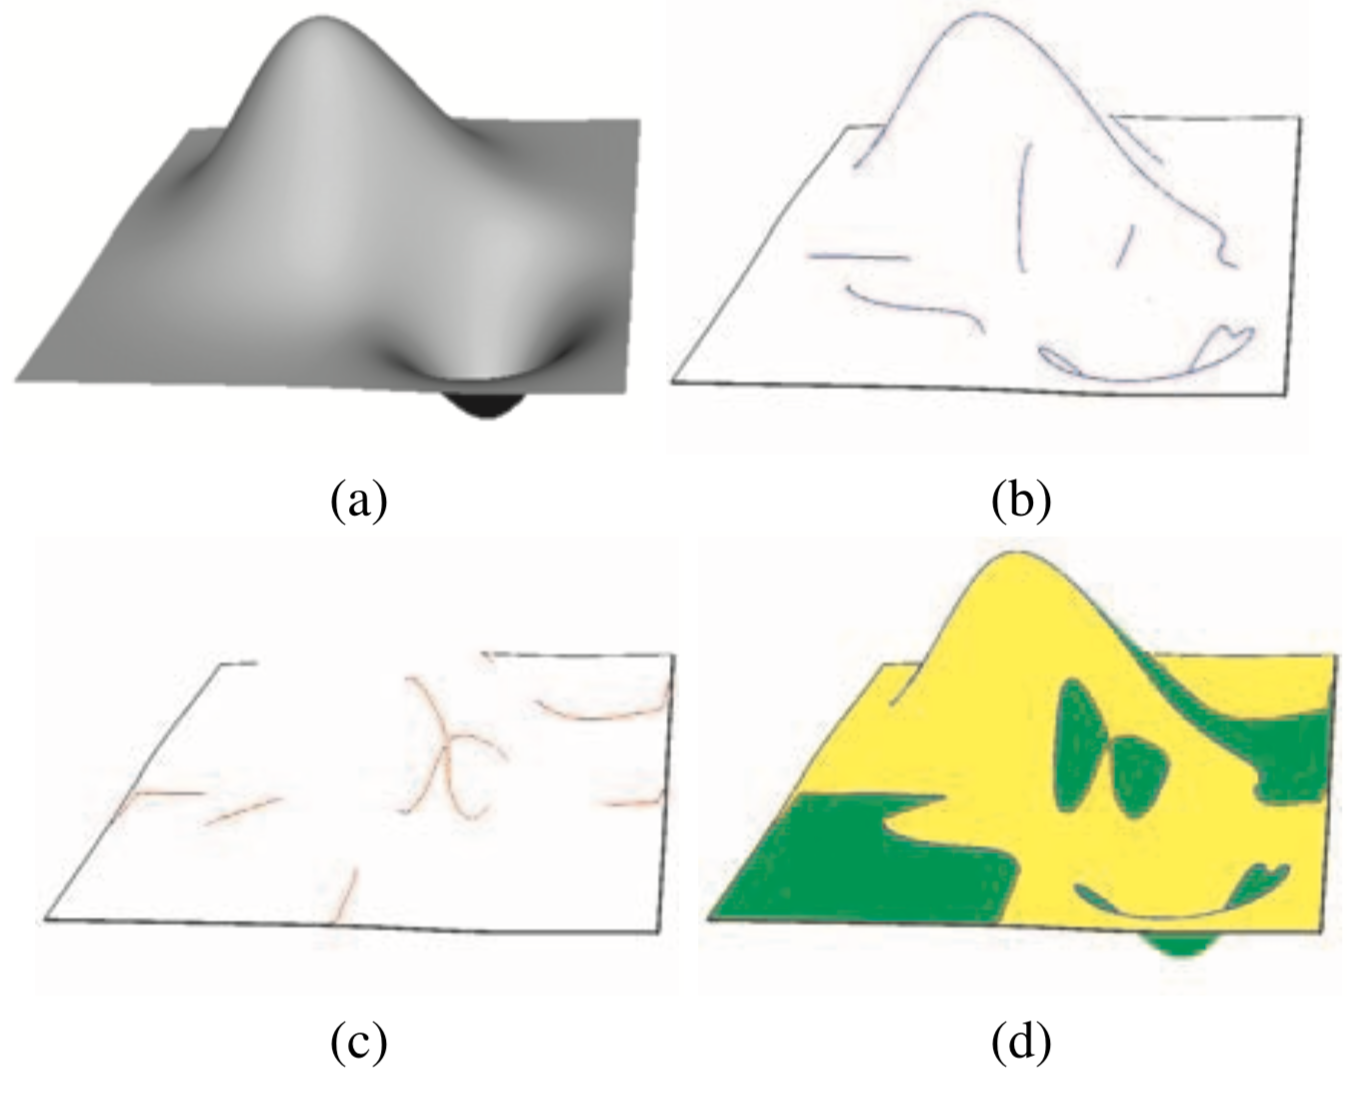
\includegraphics[width=0.7\linewidth]{abcd.png}
	\caption{(a): Die beleuchtete Oberfläche; (b): Die Maxima der zweiten partiellen Ableitung in Richtung des Gradienten. Diese werden für die PELs herausgefiltert; (c): Die Minima der zweiten partiellen Ableitung in Richtung des Gradienten; (d): Maxima und Minima ergeben geschlossene Bereiche, die sich dann in $D_{w}||\nabla f || < 0$ (gelb) und $D_{w}||\nabla f || < 0$ (grün) einteilen lassen.}
	\label{fig:abcd}
\end{figure}
\subsubsection{Beleuchtungsfunktion}
Die Grundlage für die Berechnungen der Gradienten und somit der PEL stellt die Funktion $f$ dar, die das darzustellende Objekt beleuchtet. 
Xie et al. wählen diesbezüglich das in der Computergrafik häufig verwendete Phong-Modell.
Dieses setzt sich zunächst aus drei verschiedenen Termen zusammen. Dem ambienten, dem diffusen und dem reflektierenden Term:
\begin{equation}
I = I_{amb} + I_{diff} + I_{spec}
\end{equation} 
\\\\
Aufgrund der Tatsachen, dass der ambiente Term nicht zum Unterschied in der Beleuchtung (Kontrast) beiträgt und der reflektierende Term vom Sichtvektor abhängig ist, beziehungsweise an spiegelnden Stellen entstehende Feature Lines generell wenig über die Struktur des Objekts aussagen, vereinfachen Xie et al. das Modell zu:
\begin{equation}
I = I_{diff} = k_{d}I_{d}\mathbf{n}*\mathbf{l}
\end{equation} 
\\\\
Zur Berechnung der Helligkeiten für jeden Punkt des Objekts genügen somit die Oberflächennormale $\mathbf{n}$ und der Lichtvektor $\mathbf{l}$. $k_{d}$ ist ein empirisch ermittelter Reflexionsfaktor für das Material des Objekts, $I_{d}$ ist die Lichtstärke.

\label{belfkt}
\subsubsection{Optimale Beleuchtung}
Da die Ergebnisse der PELs von der Positionierung der Lichter abhängen, schlagen Xie et al. eine von ihnen als am sinnvollsten getesteten Anordnung von Lichtern vor. Im Grunde bestehen diese aus einem Hauptlicht und optionalen Hilfslichtern.
\begin{description}
\item[Hauptlicht]\hfill \\ 
Das Hauptlicht ist ein gerichtetes Licht und beleuchtet das Objekt parallel zum Sichtvektor. Es ist zu beachten, dass dieses Licht mit der Kamera bewegt werden muss (Es entsteht eine Sicht-Abhängigkeit des Ergebnisses). \\
\item[Hilfslichter]\hfill \\
Die optionalen Spotlights sollen benutzerspezifizierte Bereiche besonders betonen. Diese sind lokal definiert und deshalb nicht von der Sicht abhängig.
\end{description}

Zur ergonomischen Positionierung der Hilfslichter wird weiterhin ein automatisches Verfahren vorgeschlagen, bei dem der Nutzer nur Bereiche des Objekts spezifizieren muss, die genauer oder weniger genau dargestellt werden sollen. Diese sind jeweils Teilmenge der gesamten Oberfläche:
\begin{equation}
\bar{S} \subseteq S
\label{eq:ssubsets}
\end{equation}
\\
Der Algorithmus sucht nun die Position $\mathbf{x}$ des Spotlights mit Richtungsvektor $\mathbf{d}$ und Zentrum der Teiloberfläche $\mathbf{c}$, sodass gilt:
\begin{equation}
\mathbf{d} = \frac{\mathbf{x} - \mathbf{c}}{||\mathbf{x} - \mathbf{c}||}
\end{equation}
und
\begin{equation}
max \int_{}\int_{\bar{S}} || \nabla f||^{2} dA 
\end{equation}
für die Maximierung, oder
\begin{equation}
min \int_{}\int_{\bar{S}} || \nabla f||^{2} dA 
\end{equation}
für die Minimierung der Beleuchtung der Teiloberfläche des Objekts. Die PELs für diese Bereiche werden dann mit den PELs des Hauptlichts ausgetauscht. 
Es lassen sich so Feature Lines, und somit Details, hinzufügen, oder entfernen (Abbildung \ref{fig:rabbit}).
\\\\
Da die Beleuchtungsfunktion $f$ stetig ist, (siehe Abschnitt \ref{defpel}) und die PELs anhand der lokalen Maxima definiert werden,
sind an den Schnittpunkten der verschiedenen Bereichen keine Unstetigkeiten und damit ungewollte Feature Lines zu erwarten (Abbildung \ref{fig:rabbit}). Schnittpunkte entstehen dort, wo Punkte aneinander grenzen, die von verschiedenen Lichtern beleuchtet werden. 
\\\\
Hervorzuheben ist, dass die Bereiche der Hilfslichter nicht von der Sicht abhängig sind und damit nur einmal berechnet werden müssen. Die Anzahl an Hilfslichtern beeinflusst also  nicht die Laufzeit einer Kamerabewegung.
\begin{figure}
	\centering
		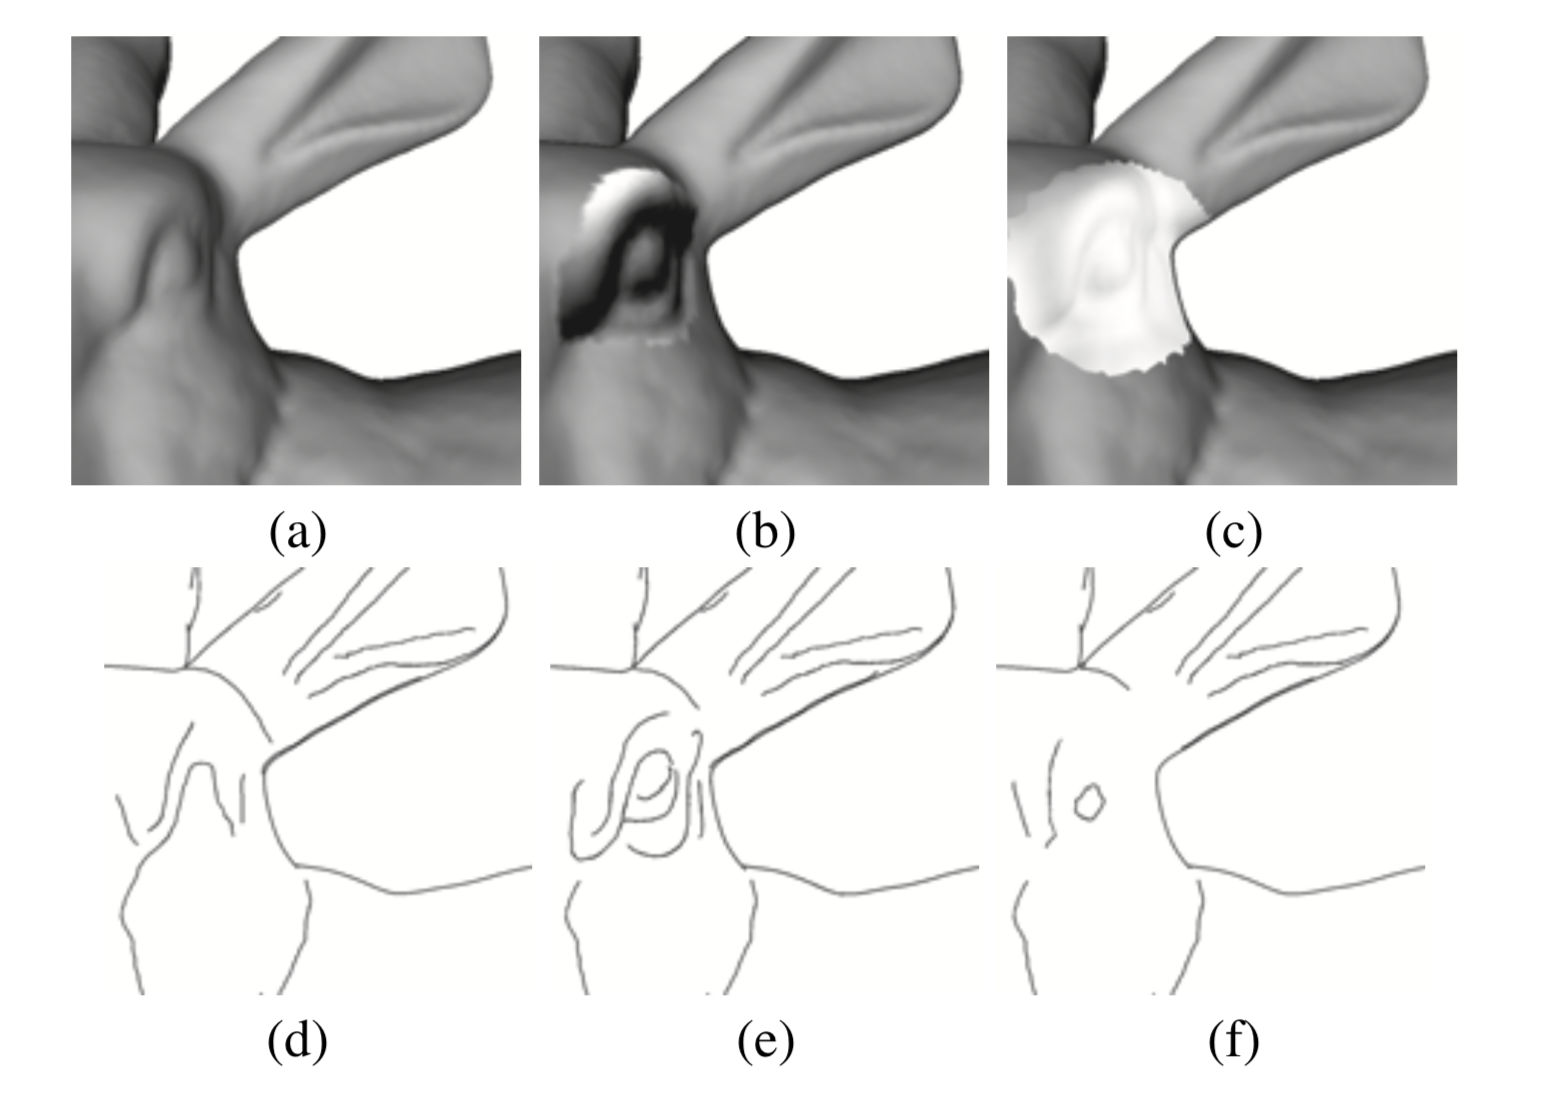
\includegraphics[width=0.7\linewidth]{rabbit.png}
	\caption{(a) und (d): Der nur durch das Hauptlicht beleuchtete Hase und zugehörige PELS. (b) und (c): Maximierung/Minimierung des Kontrasts der Beleuchtung des Bereiches um das Auge des Hasen mithilfe eines vor dem Auge positionierten Hilfslicht. (e) und (f): An den Grenzen der jeweiligen Bereiche sind in den zugehörigen PELs keine Unstetigkeiten erkennbar.}
	\label{fig:rabbit}
\end{figure}
\label{beleuchtung}
\subsubsection{Berechnung der Ableitungen}
\label{pel-impl}
Das Berechnen der (partiellen) Ableitungen bildet einen Großteil der zum Finden der PELs benötigten Schritte (vergleiche Abschnitt \ref{defpel}). Da die Oberfläche allerdings üblicherweise nicht als Funktion $S : D \subset R^{2} \longrightarrow R^{3}$, sondern als Menge einzelner Punkte gegeben ist, können Ableitungen nicht implizit berechnet werden. Xie et al. bedienen sich deshalb eines Tricks:
Die Berechnung der Ableitung eines Punktes erfolgt durch Mitteln der Ableitungen der anliegenden Dreiecke. Diese wiederum berechnen sich durch:
\begin{equation}
\resizebox{.85\hsize}{!}{$\nabla g = \left(\begin{array}{c}\frac{\partial g}{\partial x} \\ \frac{\partial g}{\partial y}\end{array}\right) = \frac{1}{d_{T}} \left(\begin{array}{rrr}y_{2}-y_{3} & y_{3}-y_{1} & y_{1}-y_{2} \\ x_{3}-x_{2} & x_{1}-y_{3} & x_{2}-x_{1}\end{array}\right) \left(\begin{array}{c}g_{1} \\ g_{2} \\ g_{3}\end{array}\right)$}
\label{eq:derivativepel}
\end{equation}
\\
$g_{1}$, $g_{2}$ und $g_{3}$ sind die Helligkeitswerte der drei Punkte des Dreiecks. Die x- und y-Werte sind die Koordinaten der Punkte im Koordinatensystem des Dreiecks und $d_{T}$ der doppelte Flächeninhalt des Dreiecks. Diese Ableitungen müssen in das jeweilige Punktkoordinatensystem überführt werden. Dies geschieht durch Multiplikation mit den Tangentenvektoren des Punktes:
\begin{equation}
\nabla g(u_{i},v_{i}) = \left(\begin{array}{c}\mathbf{u_{i}} \cdot \nabla g(x,y) \\ \mathbf{v_{i}} \cdot \nabla g(x,y)\end{array}\right)
\label{guivui}
\end{equation}
\\
Sind alle Ableitungen der anliegenden Dreiecke des Punktes berechnet und in das korrekte Koordinatensystem überführt, werden diese mittels Voronoi-Flächengewicht $w_{i}$ gemittelt und aufaddiert. Das bedeutet, dass nur der Anteil des jeweiligen Dreiecks verwendet wird, der auch am nähesten an diesem Punkt liegt. Die Ableitung eines Punktes berechnet sich demnach abschließend mittels der Formel:
 \begin{equation}
\nabla g(u,v) = \sum_{i} w_{i} \nabla g(u_{i},v_{i})
\label{guvl}
\end{equation}
 


\subsubsection{Zeichnen der PEL}
\label{zeichnen}
Um die Photic Extremum Lines abschließend zu zeichnen, müssen zunächst die Nullstellen gefunden werden, da diese zumeist nicht genau auf den Punkten des Objekts liegen. Eine Nullstelle zwischen zwei Punkten liegt genau dann vor, wenn die berechneten partiellen Ableitungen der Gradienten verschiedene Vorzeichen besitzen. Liegt eine Nullstelle vor, muss deren genauer Ort durch lineare Interpolation bestimmt werden. Dafür legen Xie et al. zunächst fest, dass $h(\mathbf{v}) = D_{w}|| \nabla f(\mathbf{v})||$. Die Interpolation ist dann gegeben durch:
\begin{equation}
\mathbf{p} = \frac{|h(\mathbf{v}_{2})|\mathbf{v}_{1}+|h(\mathbf{v}_{1})|\mathbf{v}_{2}}{|h(\mathbf{v}_{2})|+|h(\mathbf{v}_{1})|}
\end{equation}
\\
Werden zwei Nullstellen auf Kanten eines Dreiecks gefunden, kann zwischen diesen beiden Punkten eine Linie gezeichnet werden.
\\\\
Um einen Schwellwert einzubinden, der diejenigen PELs entfernt, die generell unnötige kleine Details beschreiben, wird eine Größe berücksichtigt, die sich als Stärke einer Linie betrachten lässt. Hierfür bedient sich die Gruppe einer Technik von Ohtake et al. \todo{To-Do: Quelle} und integriert $|| \nabla f ||$über die einzelnen Linien. 
\begin{equation}
\resizebox{.88\hsize}{!}{$\int{} || \nabla f ||ds \approx \sum \frac{ \nabla f(\mathbf{p}_{i})|| + || \nabla f(\mathbf{p}_{i+1})||}{2}||\mathbf{p}_{i} - \mathbf{p}_{i+1}||$}
\end{equation}
Liegt der berechnete Wert unter einem vom Nutzer gesetzten Schwellwert, wird die Linie gelöscht.
\section{Ergebnisse/Anwendungen/Diskussion}
\todo{TO-DO: Bernst und Englich - Ergebnisse/Anwendungen/Diskussion}

\begin{table}[htb]

\begin{tabular}{|l|lllll|}
\hline
 & Exp1 & Exp2 & Exp3 & Exp4 &$\theta$\\
\hline
Learning Eff. & 2 & 1 & 2 &3 & 2 \\
Usability & 2 & 2 & 3 &2 & 2.25 \\
Overview & 2 & 1 & 2 &2 & 1.75 \\
Correlat. (NT) & 3 & 2 & 3 &2 & 2.5 \\
Correlat. ( T) & 1 & 1 & 2 &2 & 1.5 \\

\hline
\end{tabular}
\caption{Eine Tabelle mit Bildunterschrift }
\label{tab:TableExample}
\end{table}

\section{Zusammenfassung/Schlussfolgerung/Ausblick}
\todo{TO-DO: Bernst und Englich - Zusammenfassung/Schlussfolgerung/Ausblick}


%-------- *.bib file with references and style file
\bibliographystyle{literaturStyle}
\bibliography{literatur}
\end{document}